%Formatting taken in part from Journal article template by Frits Wenneker at www.LaTeXTemplates.com


\documentclass[twoside,twocolumn]{article}

\usepackage{blindtext} % Package to generate dummy text throughout this template 
\usepackage{amsmath}

\usepackage[T1]{fontenc} % Use 8-bit encoding that has 256 glyphs

\usepackage{microtype} % Slightly tweak font spacing for aesthetics

\usepackage[english]{babel} % Language hyphenation and typographical rules

\usepackage[hmarginratio=1:1,top=32mm,columnsep=20pt]{geometry} % Document margins
\usepackage[hang, small,labelfont=bf,up,textfont=it,up]{caption} % Custom captions under/above floats in tables or figures
\usepackage{booktabs} % Horizontal rules in tables

\usepackage{lettrine} % The lettrine is the first enlarged letter at the beginning of the text

\usepackage{enumitem} % Customized lists
\setlist[itemize]{noitemsep} % Make itemize lists more compact

\usepackage{abstract} % Allows abstract customization
\renewcommand{\abstractnamefont}{\normalfont\bfseries} % Set the "Abstract" text to bold
\renewcommand{\abstracttextfont}{\normalfont\small\itshape} % Set the abstract itself to small italic text

\usepackage{titlesec} % Allows customization of titles
\renewcommand\thesection{\Roman{section}} % Roman numerals for the sections
\renewcommand\thesubsection{\roman{subsection}} % roman numerals for subsections
\titleformat{\section}[block]{\large\scshape\centering}{\thesection.}{1em}{} % Change the look of the section titles
\titleformat{\subsection}[block]{\large}{\thesubsection.}{1em}{} % Change the look of the section titles

\usepackage{fancyhdr} % Headers and footers
\pagestyle{fancy} % All pages have headers and footers
\fancyhead{} % Blank out the default header
\fancyfoot{} % Blank out the default footer
\fancyhead[C]{LDS TEMPLE LOCATION AND MEMBER ACCESSIBILITY $\bullet$ May 2017} % Custom header text
\fancyfoot[RO,LE]{\thepage} % Custom footer text

\usepackage{titling} % Customizing the title section

\usepackage{hyperref} % For hyperlinks in the PDF

\usepackage{tikz} % For implementing graphs
\usetikzlibrary{arrows} % Self-explanatory

\usepackage{graphicx} % Allows us to insert .png files

%----------------------------------------------------------------------------------------
%	TITLE SECTION
%----------------------------------------------------------------------------------------

\setlength{\droptitle}{-4\baselineskip} % Move the title up

\pretitle{\begin{center}\Huge\bfseries} % Article title formatting
\posttitle{\end{center}} % Article title closing formatting
\title{LDS Temple Location and Member Accessibility} % Article title
\author{%
\textsc{Applied Mathematical Modeling Research Team}\\[1ex] % Your name
\normalsize Brigham Young University  \\ % Your institution
\normalsize \href{mailto:amm@math.byu.edu}{amm@math.byu.edu} % Your email address
%\and % Uncomment if 2 authors are required, duplicate these 4 lines if more
%\textsc{Jane Smith}\thanks{Corresponding author} \\[1ex] % Second author's name
%\normalsize University of Utah \\ % Second author's institution
%\normalsize \href{mailto:jane@smith.com}{jane@smith.com} % Second author's email address
}
\date{\today} % Leave empty to omit a date
\renewcommand{\maketitlehookd}{%
\begin{abstract}
\noindent This paper uses various mathematical models to determine the best locations for LDS temples to be built within the United States in order to benefit the most members of the LDS church.
These models take into account the locations of current temples and the population density of members of the LDS church. 
The Distance Model is used to minimize the average distance from members to their nearest temple within the United States.
This investigation is followed by the Markov Chain Model.
This model accounts for the likelihood of a member attending one of the temples closest to them based off of their distance from and the busyness of each temple using a probabilistic approach.
\end{abstract}
}
% Do we need a keywords section?
\begin{document}
\maketitle


%----------------------------------------------------------------------------------------
%	ARTICLE CONTENTS
%----------------------------------------------------------------------------------------

\section{Introduction}

For members of the Church of Jesus Christ of Latter-day Saints (the LDS Church), temples are believed to be imperative in the process of gaining salvation.
Not only do members believe that temples are vital to salvation, but they also view temples as places of worship (Monson, 1995). % I feel like the ideas of these two sentences should be swapped.  I feel like being imperative to salvation is a stronger idea than just being a place of worship.  If we wanted to improve access to worship sites, we could just use church buildings.
Consequently, regular member access to temples is a high priority for the LDS Church. % Again, this feels mostly related to the salvation aspect of temples.
To maximize temple access for its members, LDS church leaders seek to find the most effective location for each temple, as constructing new temples is an expensive and time intensive process.
In the field of operations research, finding the optimal location for a new building is referred to as a facility location problem.

Location theory is a subfield of operations research that generally involves a set of demands and a set of facilities that can satisfy some of those demands (Melo, Nickel, \& Saldanha-da-Gama, 2009).
Problems in location theory want to maximize the number of demands satisfied by finding optimal locations for facilities, either through adding facilities or relocating.
There are a myriad of ways to define an optimal location, but the standard definition for median problems is a location that minimizes the average distance traveled to fulfill a demand (Owen \& Daskin, 1998).
The most prominent, and simplest, of these types of problems is the P-median problem, which tries to minimize the distance that a demand must travel to reach its nearest facility (Current, Min, \& Schilling, 1990).
Most other median problems are slight variants of the P-median problem taking into account various other parameters.

In this paper, we use mathematical models similar to those that solve variants of the P-median problem to solve the temple location problem of the LDS church.
We first use a Distance Model to determine new optimal temple locations to minimize the average distance that LDS church members must travel to their nearest temple. % Is there a standard name in the literature for a distance-based model?  I feel like calling it the "Distance Model" is a very elementary name, and if that's the current standard, then great, but it seems like there is likely another name typically used for this type of model.
This problem seeks to maximize the number of LDS members that have access to a temple measured solely by proximity to a temple.
We altered this model to use a weighted distance function to take account for behavioral choices.% Hasn't actually happened yet, but is in the works
Next, we use a Markov chains to model the likelihood of a member going to a temple using distance to and the busyness of the temples closest to that member.
This model attempts to optimize the number of LDS members that have frequent access to a temple. % Not strictly true.  Using the MFPT, we find where a new temple will decrease average distance to the temple.  Using the sum of the entries in the perron eigenvector that correspond to temples, we find where putting a new temple into the system will increase the total number of people in the temple on a given day.
Lastly, we use a ... % TODO- write about new model

The rest of the paper will be as follows.
First, Section \ref{sec:litrev} contains a review of relevant literature.
Section \ref{sec:prob} will present the problem in terms of a facility location problem.
This section will define variables and discuss assumptions made about the data gathered.
Section \ref{sec:models} will examine three modeling approaches to the problem; namely, a distance model, a Markov chain model, and ... %TODO- Decide on last model.
Section \ref{sec:res} will present the results and Section \ref{sec:analysis} will analyze the implications of the results.
Finally, Section \ref{sec:conclusion} will give a summary of the paper along with areas for further research.

\section{Relevant Literature Review}
\label{sec:litrev}
Facility location management is a well-established area within operations research.
Current, Min and Schilling report that facility location management has been researched through the perspective of many different academic disciplines.
They additionally cite one recent bibliography on the subject that had over 1500 titles, showing the vast expanse of research in this area (1990).
In their literature review, Owen and Daskin give an overview of the most used models among this immense amount of literature. 
They comment on 15 differing subsets of facility location problems, again demonstrating the voluminousness of the literature (1998).

Although the library of facility location management is vast, this review focuses primarily on literature pertaining to median problems, with a specific emphasis on using Markov chain models.
In the past, no model has been presented to optimize the placement of LDS temples, in either the United States or internationally.
Our paper seeks to fill this gap in the literature. % What a gap.  How has no one addressed  it before?  Also, we're not trying to fill the gap pertaining to international placement of temples, while this seems to imply that we are.

The study of location theory began with Alfred Weber in 1909. % How much of a history lesson is required for a literature review?
He researched where to place a warehouse based off of the average distance that would be traveled by those who would need to visit the warehouse (Owen \& Daskin).
This research created the basis for {\em median problems}, or problems to determine a facility location by minimizing the average distance traveled by consumers. % (suggested) With distance being a function of various variables i.e. actual distance, traffic, busyness, proximity to competitors, etc.
As noted by Melo, Nickel and Saldanha-da-Gamma, the p-median problem is considered the simplest and most prominent median problem.  % This is almost exactly restating line 93 of this paper with a different source.  One of the lines should probably go or we can choose adjectives other than simplest and most prominent to describe the p-median problem.
They define the p-median problem as the problem where p facilities need to be placed to minimize the total weighted distance or costs to satisfy customer demands (2009).

From the simplest definition of p-median problems arises a myriad of slight variations of it to account for the context of the problem. % I thought the p-median problem was the simplest median problem?  Is there more than one original p-median problem?
For example, Berman, Drezner, and Wesolowsky use a model formulation which allows demands to be serviced by facilities other than the one closest to them (2003). % Is this relevant to our paper?  If so, how?
In their review, Current, Min, and Schilling found that 33 out of 45 articles revealed dealt with a variation of a p-median problem.

Once a median problem has been formulated, a portion of literature furthers models the problem using a network of nodes.
Bruni, Beraldi, and Conforti use an undirected graph to model a complex water distribution network (2016).
Similarly, Jouzdani, Sadjadi, Fathian model a dairy production network with a directed graph.
They use actual nodes to denote potential facility locations and virtual nodes to denote the sink and source nodes for each product (2013).

Not only are they frequently used, but networks have been highly researched within location theory.
In their article, Ottaviano and Thisse define a network as a finite, connected set of arcs in a plane of well-defined length.
They let the nodes in the network denote potential facility locations (2004). % We're not doing anything similar to this.  I don't know much about how a lit review is meant to be written, but it seems like what we talk about should be directly related to our research.

% I don't know if this is a problem, but in this section, the first four paragraphs don't have a space separating them, but the last 3 do.  I don't know enough about latex to try and fix it, though...

...
% TODO- Now talk about how Hakimi proved that there exists an answer to the p-minimization problem given this formulation
% Then transition in Markov chains for the last part of the literature review.

\section{Problem Formulation}
\label{sec:prob}

Our problem can be formulated in two main ways. % It doesn't really feel like two ways...
The first is the problem of maximizing the number of LDS church members that have access to the temple (could be one-time access). % If you define access as being close.  We're really minimizing the average distance to the temple each member has to travel.
The second is to maximize the number of members that have frequent access to the temple. % Or regular access?  We've kind of dictated the frequency people attend the temple.  I'm not sure that this is an accurate differentiation between the two ways our problem can be formulated.  I feel like we're maximizing the same thing, we're just using a different way to calculate it.
In order to define our models, we delineate our variables.
We will then explain the assumptions that we made in our models in order to simplify them.

\subsection{Important Variables}
\begin{tabular}{c | l}
Variable & Description\\
\hline
$d(s_{i},t_{j})$ & Distance from stake $s_{i}$ to temple $t_{j}$\\
$\rho_{i}$ & Density of stake $s_{i}$\\
$S$ & Set of all stakes\\
$s_{i}$ & Stake number $i$\\
$T$ & Set of all Temples\\
$T_{new}$ & The proposed new temple location\\
$t_{i}$ & Temple number $i$ \\
$\tau_{i}$ & Temple score of temple $t_{i}$\\
\end{tabular}
\vspace{0.1in}

% I don't know what the standard is, but it might be nice to define the variables in the same order in which we explain them below.

\noindent To fully understand our approach, it is crucial to know what factors were considered relevant, and which were excluded. % Do we need to discuss what we excluded from our analysis?
Chief among these factors is the distance $d(s_{i},t_{j})$ from a stake center to a temple.
This distance is measured using the Vincenty Algorithm in order to account for the shape of the earth and give very accurate measurements based on latitude and longitude.
While this may be sufficient for the distance model, a fair number of other considerations were necessary for the Markov chain model and the ...
For the Markov chain model, we included a measure of the busyness for each temple.
To do this, we gave each temple a score, $\tau_{i}$, based on the number of stakes that listed that temple as one of its five closest temples, determined by Euclidean distance.
Using these scores, we assigned each stake a density $\rho_{i}$, that sought to relate how much traffic each stake would provide to its surrounding temples.
This allowed us to approximate how busy a temple was, using the stakes that consider it one of their closest temples.
We also used the Markov model where we neglected the busyness of each temple and replaced it with a function of distance where a far temple would discourage people from attending. % Is here the appropriate place to include the function?  Or in a later section?
For the ... model, we ...

\subsection{Assumptions and Data}
To simplify the models and make an analytical review of temple location optimization possible, a number of assumptions were made.
Firstly, it is assumed that every LDS stake in the United States has the same number of active, temple-going members contained within its boundaries.
This approximation, combined with the assumption that every stake center is located near the center of the stake, allows us to estimate the member density throughout the country.
Within each model, further assumptions are made regarding the proportion of members that attend daily from each stake, and how the distance and busyness of each temple affects these proportions, but these details will be clarified for each individual model.

\section{Modeling Approaches}
\label{sec:models}
This section is a mathematical explanation of the assumptions made and the models used.
As choosing the location of an LDS temple mathematically involves various assumptions about human behavior, as well as several possible objectives, we separate our explanation of the models used to solve this problem into subsections. % Do we need an explanation about why we used subsections?  It feels self-evident.
Each subsection is self-contained in the assumptions made and the problem setup.
Along with the individual models presented in each subsection, there is also a brief summary of the algorithmic approach used to find the optimal solution to each.

\subsection{Distance Model} 

The simplest model used is the Distance Model (DM).
The purpose of DM is to minimize the average distance a given member of a LDS stake has to travel to get to their closest temple.% Is this just the p-median problem?  Are there notable differences we should bring up?
As such, this model does not take into account the capacity of the temples, nor the relative accessibility of other temples, even if they are a similar distance away. % Do any of our models take into account the capacity of the temple?
The only assumption made about the behavior of church members are that they desire to have a temple close to their stake center, and that they will only use the closest temple to them.

The mathematical setup is as follows. Let each stake be represented as $s_i$ and each temple $t_j$, and let the set of all the stakes be represented as $S$ and likewise the temples as $T$.
The average distance a given member of an LDS stake has to travel to get to their closest temple is:

\begin{equation}
	f(S,T) = \sum_i \underset{j}{\text{min}}\{d(s_i,t_j)\}.
\end{equation}

The unconstrained optimization problem can then be written as:

\begin{equation}
\begin{aligned}
	\underset{T_{new}}{\text{Minimize }} f(S,T^*), \text{ where } T^* = T \cup T_{new}.
\end{aligned}
\end{equation}

In this model, we only considered $T_{new}$ with carnality 1; that is, we assume only one temple;s location is to be determined at a time. 
This is for convenience of calculation, as the LDS church often decides to build multiple temples in a year. % We could include this in further research

To maximize the objective function, we used a pseudo Monte Carlo method in which we divide the United States into one million evenly spaced points and evaluated the objective function at that point.
We assumed the objective function is smooth, so following that we looked more closely at the places at which our model indicated there was need of a temple % to be deleted if we don't do further analysis as suggested by Dr. Jarvis.  Also, do we have some slick justification behind the smoothness of the objective function?


\subsection{Markov Modeling}

Markov chains are used in a myriad of fields
 For the purposes of this study, Markov chains are useful because they reveal the effects that simple local behaviors have on more complex global behaviors.
Specifically, the effects of the busyness of each individual temple on the members that live nearby it can be modeled on a more global level.
While Markov chains do not predict individual behavior very accurately, they are very powerful when observing on the aggregate, which is exactly what we want.

This section gives a brief outline of key characteristics of a Markov chain and then the specific application of those in this model.

\subsubsection{Background}

A Markov chain is an example of a stochastic simulation of a $n$ state closed system. % How much background do we want to include?  We don't want to copy the paper we're basing this off.
We create an $n\times n$ matrix $P$ where $p_{i,j}$ represents the probability of moving from state $i$ to state $j$.
We observe that in each time step, the probability that a person moves from state $i$ to another state in the system is 1 because we have a closed system.
This means that each row in our transition matrix should have sum equal to one, which is known as {\em row stochastic}.

One of the powerful applications of Markov chains is that we can simulate what happens to a starting position.
We can model any starting point as a vector $x_0$ and see what happens after one time step by letting $x_1 = P x_0$.
More generally, we say $x_{n + 1} = P x_n$.
Because we have a row stochastic matrix, we can see that the all-ones vector is an eigenvector of $P$, which implies that the spectral radius is 1. % Needs smoothing, maybe an additional sentence.
% Include hypothesis of Perron Frob. theorem?
The Perron Frobenious Theorem tells us that in this case, the dominant left eigenvalue is 1, it has an all-positive eigenvector, and it represents the steady state of the system.
This eigenvector is known as the Perron eigenvector and is important for our analysis of the model.

\subsubsection{Model}
The second model used is closely based on the Markov chain application of Faizrahnemoon, Schlote, Maggi, Crisostomi, and Shorten (2015).
It involves two stages: the initialization of the model transition matrix and the computation of the Perron eigenvectors, Mean First Passage Time, and Kemeny constant described above.
To understand this concept more fully, we consider a graph in which each stake is connected to the two closest temples as shown in \ref{fig:M1}.\newline

% If we want a figure to demonstrate every stake and its five closest temples, that's in Testing.ipynb.  It's a messy graph, though.

% Create a figure to demonstrate stakes connected to 2 closest temples | Also in Testing.ipynb.

% This code is based off of https://tex.stackexchange.com/questions/45734/drawing-graphs-in-latex
%        as well as https://tex.stackexchange.com/questions/24000/how-to-add-caption-for-a-tikz-picture
\begin{figure}[h!]
\centering

\begin{tikzpicture} [->, >=stealth' ,shorten >=1pt, auto,node distance=2.25cm,thick,main node/.style={circle,draw,font=\sffamily\Large\bfseries}]
\node[main node] (1) {$T_{1}$}; % Creates a node referred to as (1) with label T_1
\node[main node] (2) [below left of=1] {$S_{1}$}; % Creates the node and positions it
\node[main node] (3) [above right of=1] {$S_{5}$};
\node[main node] (4) [right of=1] {$S_{4}$};
\node[main node] (5) [below right of=1] {$S_{3}$};
\node[main node] (6) [right of=4] {$T_{2}$};
\node[main node] (7) [above of=6] {$S_{6}$};
\node[main node] (8) [below right of=5] {$T_{3}$};
\node[main node] (9) [below of=1] {$S_{2}$};
\node[main node] (10) [below of=6] {$S_{7}$};

\path[every node/.style={font=\sffamily\small}]
(2) edge node [right] {0.6} (1) % Adds an edge from node (2) to node (1) with the label of 0.6 on the right of the edge
(2) edge [bend right] node [left] {1.5} (8) % Adds a curved edge from node (2) to node (1) with the label of 1.5 on the left of the edge
(3) edge node[left] {0.4} (1)
(3) edge [bend left] node [right] {1.2} (6)
(4) edge node [above] {0.2} (1)
(4) edge node [above] {0.4} (6)
(5) edge node [right] {0.3} (1)
(5) edge node [right] {0.3} (8)
(7) edge node [right] {1.6} (1)
(7) edge node [right] {0.7} (6)
(9) edge node[right] {0.4} (1)
(9) edge node [above] {1.2} (8)
(10) edge node [right] {0.8} (6)
(10) edge node [above] {0.2} (8);
\end{tikzpicture}

\caption{A sample graph including $7$ stakes and $3$ temples. \textbf{Note}: Edges in this figure are a measure of distance, not a measure of probability.} % Maybe edges should correspond to probability?
\label{fig:M1}
\end{figure}
% End code for graph

In order to begin creating this model, we initialize a square probability matrix $T$ of zeros in which the first $n$ rows and columns correspond to the church stakes in the United States and the next $m$ rows and columns correspond to the church temples in the United States.
Each $t_{ij}$ in the matrix represents the probability that a person in row $i$ will travel to column $j$ in the current state. The diagonal entries $t_{ii}$ represent the probability that a person will remain in their current location through the current state.
The states of the matrix represent a single day.
% Create a visual matrix representation of the matrix initialized | There's a version where the magnitude of the entry is color in No_Busyness_Test.ipynb

We begin populating the matrix by allowing the diagonals $t_{ii} = 29/30$ which numerically represents the assumption that in each state or day, $1/30$ of a stake's active temple attendees will attend the temple.
We then adjust this number with a measure of a stakes relative busyness in a single day.
To do so, we compute a measure of busyness by taking into account the number of stakes within a close proximity to each temple.
The required numerical representations are described below.

\begin{equation}
\begin{aligned}
Ts_j = \sqrt{1\over{\sum_j{t_{ij}}}}
\end{aligned}
\end{equation}


\subsection{Last Model} % TODO- figure out last model. Once updated the paper overview in the introduction will need to be updated.
Insert text here.

\section{Results}
\label{sec:res}
Insert text here.

\subsection{Distance Model}
After running the Distance Model on one million points, we graphed the data for ease of analysis.
In Figure 2, the magnitude of the reduction on total distance traveled by members of the LDS church is graphed on top of the United States for convenience of interpretation.
The darker regions correspond to a greater impact on distance traveled.
We can see that our model advises us to build a temple in northeastern Oklahoma or northwestern Arkansas.
% Do we need to discuss other locations suggested by the model?  What else is "Results" for this model?

% I didn't know which figure we were going to need, so I included both of them. | The first one's fine.  They are the same data graphed using a slightly different maximum.
% NOTE : If viewing with overleaf, images can not be found, so do not include this code.
\begin{figure}[h!] % The [h!] forces LaTeX to put the figure right where it appears in the text.
\centering % Center it based on the text
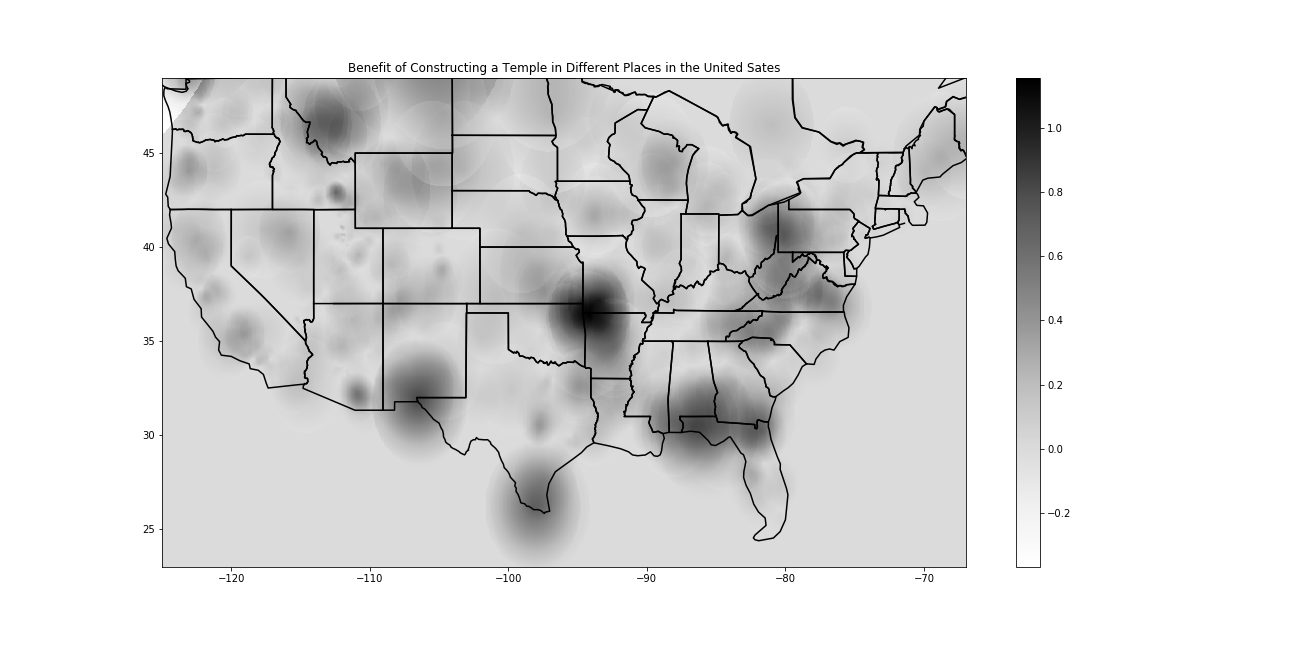
\includegraphics[width=0.6\textwidth]{Euclidean_Graph1} % Loads and scales the image
\caption{Results : Distance Model} % Adds a caption
\label{fig:Results1}
\end{figure}

%\begin{figure}[h!]
%\centering
%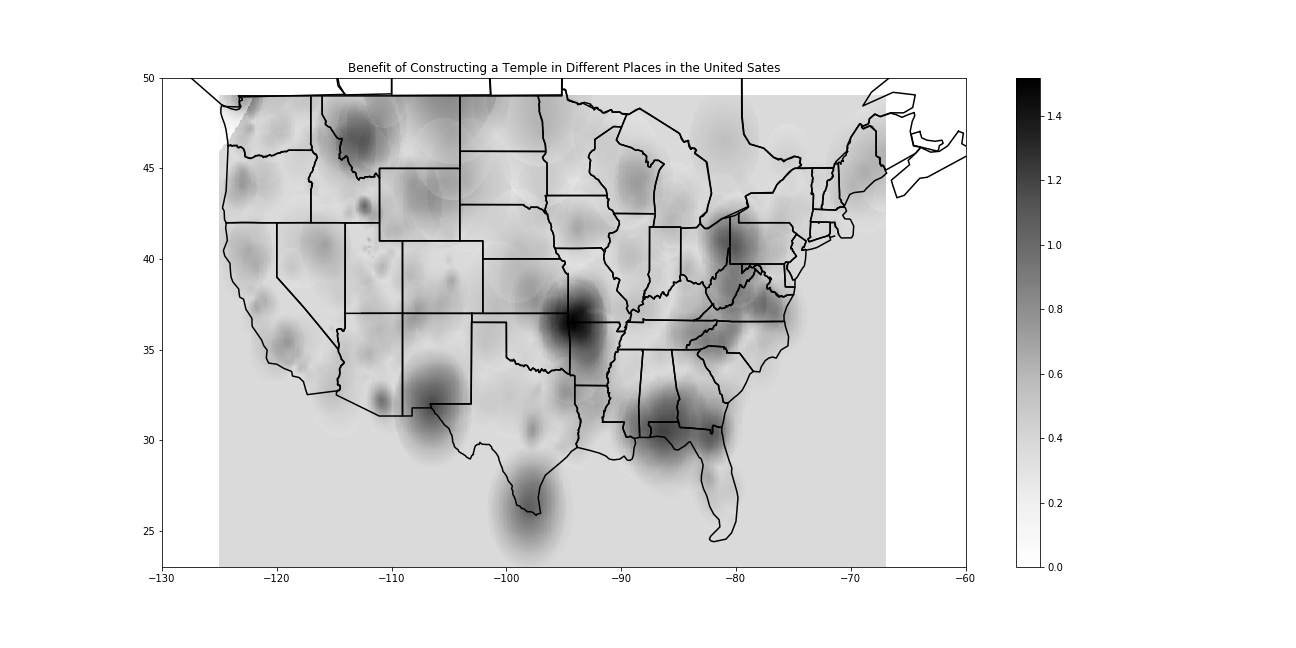
\includegraphics[width=0.6\textwidth]{Euclidean_Graph2}
%\caption{Euclidean Graph 2}
%\label{fig:Results2}
%\end{figure}
% End of image importing
% We should change the title of the graph to reflect that we're using the Distance model.  We should also remove the legend because it doesn't lend any useful information.  We could also get a basemap plot which would look a lot nicer.  We also may want to include the stake and temple locations on the graph.  It also might be nice to have a slightly larger graph so it is clearer to see.

\subsection{Markov Model}
Insert text here.

\subsection{Last Model}
Insert text here.

\section{Analysis}
\label{sec:analysis}
Insert text here.

\section{Conclusion}
\label{sec:conclusion}
Insert text here.

%----------------------------------------------------------------------------------------
%	REFERENCE LIST
%----------------------------------------------------------------------------------------

\begin{thebibliography}{99} % Bibliography - this is intentionally simple in this template
% Below is an example
%\bibitem[Crisostomi, Kirkland and Shorten, 2011]{Crisostomi:2011dg}
%Crisostomi E, Kirkland S, Shorten R. 
%\newblock A Google-like model of road network dynamics and its application to regulation and control.
%\newblock {\em Int. J. Control.} 2011;84:633--651.

\bibitem[Berman, Drezner, Wesolowsky, 2003]{Berman:2003}
Berman O, Drezner Z, Wesolowsky G.
\newblock Locating service facilities whose reliability is distance dependent.
\newblock {\em Computers \& Operations Research.} 2003; 30:1683-1695.

\bibitem[Bruni, Beraldi, Conforti, 2016]{Bruni:2016}
Bruni M, Beraldi P, Conforti D.
\newblock Water distribution networks design under uncertainty.
\newblock {\em TOP.} 2016; 25:111-126.

\bibitem[Current, Min, Schilling, 1990]{Current:1990}
Current J, Min H, Schilling D.
\newblock Multiobjective analysis of facility location decisions.
\newblock {\em European Journal of Operational Research.} 1990; 49:295-307.

% This reference was taken out of the introduction
%\bibitem["Facts and Statistics", 2017]{Facts&Stats:2017}
%\newblock 2017; Retrieved from http://www.mormonnewsroom.org/facts-and-statistics

\bibitem[Faizrahnemoon, Schlote, Maggi, Crisostomi, Shorten, 2015]{Faizrahnemoon:2015}
Faizrahnemoon M, Schlote A, Maggi L, Crisostomi E, Shorten R.
\newblock A big-data model for multi-modal public transportation with application to macroscopic control and optimisation
\newblock {\em International Journal of Control.} 2015; 88:2354-2368.

\bibitem[Jouzdani, Sadjadi, Fathian, 2013]{Jouzdani:2013}
Jouzdani J, Sadjadi S, Fathian M.
\newblock Dynamic dairy facility location and supply chain planning under traffic congestion and demand uncertainty: A case study of Tehran
\newblock {\em Applied Mathematical Modeling.} 2013; 37: 8467-8483.

\bibitem[Melo, Nickel, Saldanha-da-Gama, 2009]{Melo:2009}
Melo M, Nickel S, Saldanha-da-Gama F.
\newblock Facility location and supply-chain management - A review.
\newblock {\em European Journal of Operational Research.}  2009; 196:401--412.

\bibitem[Monson, 1995]{Monson:1995}
Monson T.
\newblock Blessings of the Temple. 1995;
\newblock Retrieved from https://www.lds.org/church/temples/why-we-build-temples/blessings-of-the-temple?lang=eng

\bibitem[Ottaviano, Thisse, 2004]{Ottaviano:2004}
Ottaviano G, Thisse J.
\newblock New Economic Geography: What about the N?
\newblock Paper provided by Universite/ catholique de Louvain, Center for Operations Research and Econometrics in its series {\em Core Discussion Papers}. 2004065.

\bibitem[Owen, Daskin, 1998]{Owen:1998}
Owen S, Daskin M.
\newblock Strategic facility location: a review.
\newblock {\em European Journal of Operational Research.} 1998; 111:423-447.

% This section was taken out of the introduction.
%\bibitem["Statistics", 2017]{Stats:2017}
%\newblock 2017; Retrieved from http://www.ldschurchtemples.com/statistics/

\end{thebibliography}

%----------------------------------------------------------------------------------------

\end{document}